\documentclass[border=2pt]{standalone}
\usepackage{tikz}
\usetikzlibrary{arrows.meta,decorations.pathreplacing,positioning,calc}
\usepackage{amsmath}
\usepackage{helvet}
\usepackage{sansmath}

\begin{document}
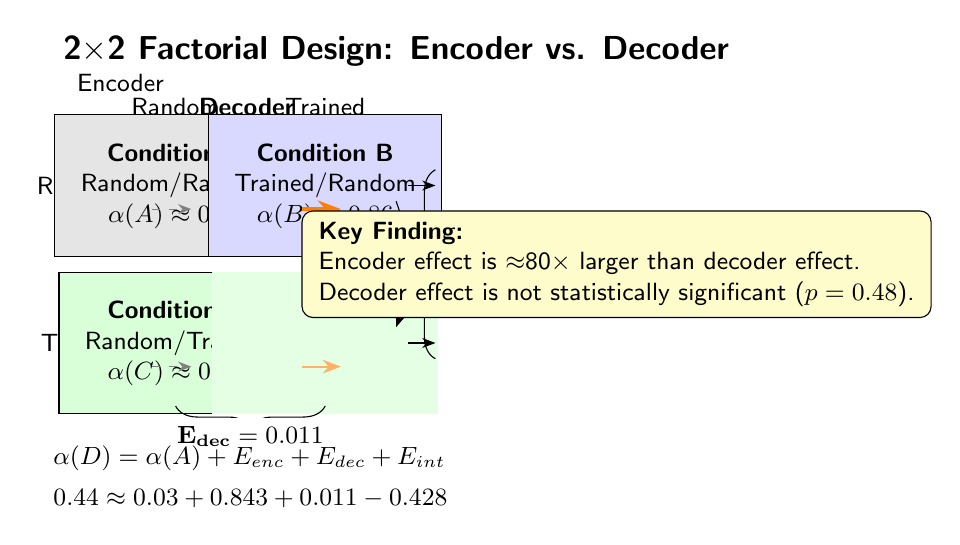
\begin{tikzpicture}[
  quad/.style={draw, minimum width=2.2cm, minimum height=1.8cm, align=center, font=\sffamily\small},
  node/.style={circle, draw, minimum size=0.5cm, font=\sffamily\tiny, inner sep=0.1pt},
  feat/.style={circle, draw, minimum size=0.35cm, font=\sffamily\tiny, inner sep=0pt},
  arr/.style={->, >=Stealth},
  every pin edge/.style={arr, dashed, gray},
  brace/.style={decoration={brace, amplitude=8pt, mirror}, decorate},
]

% Title
\node[font=\sffamily\bfseries\large] at (0, 4.2) {2$\times$2 Factorial Design: Encoder vs. Decoder};

% Column headers
\node[font=\sffamily\small\bfseries] at (-1.9, 3.5) {Decoder};
\node[font=\sffamily\small] at (-3.5, 3.8) {Encoder};
\node[font=\sffamily\small] at (-2.8, 3.5) {Random};
\node[font=\sffamily\small] at (-0.9, 3.5) {Trained};

% Row labels
\node[font=\sffamily\small] at (-4.0, 2.5) {Random};
\node[font=\sffamily\small] at (-4.0, 0.5) {Trained};

% Quadrant A (Random, Random)
\node[quad, fill=gray!20] (A) at (-2.8, 2.5) {%
  \begin{tabular}{c}
  \textbf{Condition A} \\
  Random/Random \\
  $\alpha(A) \approx 0.03$
  \end{tabular}};
\draw[arr, dashed, gray] (-3.1, 2.2) -- (-2.6, 2.2);

% Quadrant B (Trained, Random) - encoder drives absorption
\node[quad, fill=blue!15] (B) at (-0.9, 2.5) {%
  \begin{tabular}{c}
  \textbf{Condition B} \\
  Trained/Random \\
  $\alpha(B) \approx 0.86$
  \end{tabular}};
\draw[arr, very thick, orange] (-1.2, 2.2) -- (-0.7, 2.2);
\node[font=\sffamily\small, orange!60!black, below=0.1 of B] {Strong absorption};

% Quadrant C (Random, Trained)
\node[quad, fill=green!15] (C) at (-2.8, 0.5) {%
  \begin{tabular}{c}
  \textbf{Condition C} \\
  Random/Trained \\
  $\alpha(C) \approx 0.03$
  \end{tabular}};
\draw[arr, dashed, gray] (-3.1, 0.2) -- (-2.6, 0.2);

% Quadrant D (Trained, Trained) - full training
\node[quad, fill=blue!10, green!10] (D) at (-0.9, 0.5) {%
  \begin{tabular}{c}
  \textbf{Condition D} \\
  Trained/Trained \\
  $\alpha(D) \approx 0.44$
  \end{tabular}};
\draw[arr, thick, orange!60] (-1.2, 0.2) -- (-0.7, 0.2);

% Encoder effect bracket (right side, spanning B and D)
\draw[brace] (0.5, 2.7) -- (0.5, 0.3) node[midway, right=4pt, font=\sffamily\small, fill=white] {$\mathbf{E_{enc} = 0.843}$};
\draw[arr, <-] (0.5, 2.5) -- (0.15, 2.5);
\draw[arr, <-] (0.5, 0.5) -- (0.15, 0.5);

% Decoder effect bracket (bottom, spanning C and D)
\draw[brace] (-2.8, -0.3) -- (-0.9, -0.3) node[midway, below=4pt, font=\sffamily\small, fill=white] {$\mathbf{E_{dec} = 0.011}$};

% Decomposition formula
\node[font=\sffamily\small, align=left] at (-1.85, -1.2) {%
  $\alpha(D) = \alpha(A) + E_{enc} + E_{dec} + E_{int}$ \\[4pt]
  $0.44 \approx 0.03 + 0.843 + 0.011 - 0.428$
};

% Arrow from B to D (decoder disentanglement)
\draw[arr, ->, bend left=20] (0.0, 2.3) to node[right, font=\sffamily\tiny] {Decoder\\disentangles} (-0.0, 0.7);

% Key insight box
\node[draw, fill=yellow!20, rounded corners, font=\sffamily\small, align=left, inner ysep=4pt, inner xsep=6pt] at (2.8, 1.5) {%
  \textbf{Key Finding:} \\
  Encoder effect is $\approx$80$\times$ larger than decoder effect. \\
  Decoder effect is not statistically significant ($p=0.48$).
};

\end{tikzpicture}
\end{document}